\chapter{Evaluation}\label{chap:evaluation}
The contribution of this thesis is the direct comparison of the network architectures presented in the previous section on data from the Business Process Intelligence Competitions 2011 and 2012~\cite{BPIC2011, BPIC2012}. The execution of this comparison in code, the preceding data preparation and transformation as well as the obtained results shall be presented in this chapter.

\section{Used Technologies}
Anaconda~\cite{web:anaconda} was set up to create a stable working environment in which dependencies and libraries would not change.
Then, the data was explored, prepared and cleansed in an iterative fashion using JupyterLab notebooks~\cite{web:jupyter}. Helpful libraries in the process were prefixspan-py~\cite{web:prefixspan-py} and OpyenXes~\cite{web:opyenxes}. Notebooks were also used to develop the ANN training code in Keras~\cite{web:keras}.

As the codebase became more mature, Docker containers were built with the Anaconda environment inside them~\cite{web:docker}. Using a version of Docker for GPU applications running on NVIDIA hardware~\cite{web:nvidia-docker}, the networks were trained on the GPU cluster infrastructure of the HPI FutureSOC Lab~\cite{web:fsoc}. The complete source code is available for download at: \url{https://github.com/flxw/master-thesis-code}.

\section{Data preprocessing}
Following the KDD process~\cite{fayyad1996data}, the data was preprocessed to eliminate generally known properties that hinder machine learning model performance. Here, this encompassed two steps for both datasets:

\begin{enumerate}
    \item All columns which exhibited zero entropy, i.e. which were constituted of a single value, were dropped.
    \item Features which correlated strongly were eliminated. To account for categorical ones, the bias-corrected version of Cramér's~V~\cite{bergsma2013bias} was used.
\end{enumerate}


For both BPIC2011 and BPIC2012 datasets, the column \texttt{lifecycle:transition} was dropped in step 1. To make statements about upcoming workflow-related activities only, only completion events related to workflow activities were kept in the BPIC2012 log \cite{evermann2016}.

In step 2, the bi-directional results in \autoref{fig:bpic2011-correlation-heatmap} from Cramér's V revealed that the variables \texttt{Producer code}, \texttt{Activity code} and \texttt{Specialism code} correlate strongly with many others in the BPIC2011 dataset. Thus, these were dropped. As evidenced in \autoref{fig:bpic2012-correlation-heatmap}, the BPIC2012 dataset with its small number of features did not require any removals.

\begin{figure}
\centering
\subfloat[][BPIC2011 Cramér's V heatmap]{
    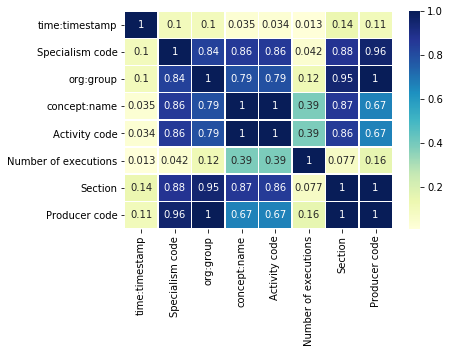
\includegraphics[width=0.5\textwidth]{gfx/bpic2011-correlation-matrix.png}
    \label{fig:bpic2011-correlation-heatmap}
}
\qquad
\subfloat[][BPIC2012 Cramér's V heatmap]{
    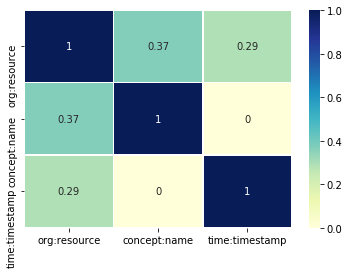
\includegraphics[width=0.35\textwidth]{gfx/bpic2012-correlation-matrix.png}
    \label{fig:bpic2012-correlation-heatmap}
}
\caption{Correlation heatmaps with values from Cramér's V.}
\end{figure}

\section{Data transformation}
Having removed unneeded features, the remaining ones were encoded following standard practice. Each numerical feature $x$ was normalized for with values specific to each trace using the min-max method:

$$normalize(x) = \frac{x-min(x)}{max(x)-min(x)}$$
\todo[inline]{Revisit this when benchmarks are through}

Categorical features without ordinal properties, which were all of them, were encoded using one-hot encoding if possible. In the case of the input for Evermann's model, they were encoded with dictionary encoding, as this encoding is required for Embedding layers.

\subsection*{SP-2 feature engineering}
The SP-2 features were engineered in an iterative fashion, as \autoref{lst:sp2-generation} outlines. For every trace, a new data frame \texttt{sp2\_df} is created and the occurence of the first activity is marked inside it. For all following activities, the contents of the previous row inside \texttt{sp2\_df} are copied into the current one and the presence of the current activity is marked. This repeats itself until the trace has been processed completely.

\begin{lstlisting}[caption={SP-2 feature generation algorithm for a single trace},label={lst:sp2-generation}]
sp2_df = pd.DataFrame(columns=activity_labels, index=range(0,len(t)), dtype=np.bool)
for col in sp2_df.columns: sp2_df[col].values[:] = 0
sp2_df["{0}{1}".format(sp2_prefix, t["concept:name"][0])].values[0]  = 1

for i in range(1,len(t)):
    first_activity_name = t["concept:name"].iloc[i]
    col = "{0}{1}".format(sp2_prefix,first_activity_name)
    
    sp2_df.values[i] = sp2_df.values[i-1]
    sp2_df[col].values[i] = 1
\end{lstlisting}

\subsection*{Sub-sequence feature engineering}
The sub-sequence features for the PFS model were created with the help of the \textit{prefixspan-py} library~\cite{web:prefixspan-py}. As \autoref{lst:pfs-mining} shows, the library greatly facilitates obtaining closed sequences ranked by support and returns a two-dimensional array of sub-sequences. This array contains one array per sub-sequence.
\todo[inline]{put closed sequences and support into background}

\begin{lstlisting}[caption={Obtaining closed sequences using the \textit{prefixspan-py} library.}, label={lst:pfs-mining}]
prefixspan_traces = PrefixSpan(encoded_traces)
closed_sequences = prefixspan_traces.topk(25, closed=True)
\end{lstlisting}

After mining the sequences, a loop is executed for every trace, shown in \autoref{lst:subsequence-feature-creation}. The activity at the current index is compared with the beginning of every subsequence in the list of subsequences. If they are equal, the foremost activity of that subsequence is popped. Should this depletes the list, the subsequence is consideres as completely occured and is marked as such. This continues until the end of every trace.

\begin{lstlisting}[caption={Creating the subsequence features.}, label={lst:subsequence-feature-creation}]
col_prefix = "PFS_"
subseq_labels = [ "{0}{1}".format(col_prefix,ss_idx) for ss_idx, ss in enumerate(ps) ]
subseq_df = pd.DataFrame(columns=subseq_labels, index=range(0,len(t)))

for col in subseq_df.columns: subseq_df[col].values[:] = 0
for i in range(0,len(t)):
    activity_code = t["concept:name"].iloc[i]
    
    for subseq_idx in range(0,len(ps)):
        if ps[subseq_idx] == []:
            continue
        if ps[subseq_idx][0] == activity_code:
            ps[subseq_idx].pop(0)
            if ps[subseq_idx] == []:
                subseq_df.values[i:,subseq_idx] = 1
\end{lstlisting}

\todo[inline]{Choosing a specific support for the PFS features...}

\section{Technical considerations}
The prediction task at hand was framed as a multi-class classification problem with a time-component, as a class for the next activity needed to be predicted using a variable amount of input. Extensive use was made of Keras' LSTM layers, which led to the implementation decision in the following:\\

As weights are updated after every batch, the batch size is an important parameter. Typical machine learning algorithm inputs are rows where each rows and its corresponding prediction target stand for themselves. In the case presented here, the time-steps of a sequence do build upon each other, and training on multiple unrelated sequences with variable timesteps makes a semantic separation of unrelated data, so that there is no?!?!

This was achieved by leveraging three-dimensional vectors to feed data into the network. Each dimension can be understood as follows:

\begin{enumerate}
    \item Number of sequences per batch
    \item Number of time-steps per sequence
    \item Number of variables per time-step
\end{enumerate}

This definition demands a design choice as Keras requires the number of time-steps inside batch to be constant. Three approaches are thinkable:\\

First, padding all sequences to the same length with null values which RNNs were supposed to be capable of understanding as such. Several forums suggest doing so, but as no hard evidence could be found, this approach was forgone.

Secondly, grouping training traces by length and thus modifying the first dimension of the input vector, the number of sequences per batch. This would reduce the number of batches from 900 to 310 on the BPIC2011 training set, leveraging the power-law distribution in trace lengths, clearly evidenced in \autoref{fig:bpic2011-length-distribution}.

Third and most straightforward, training one sequence per batch. These last two approaches shall be evaluated for impact on each network.

\section{Test setup}
Dropping the embedding layer if results are really bad
Iterative way of working, these are the ultimate results
Making embedding layer optional

\begin{table}[]
    \centering
    \begin{tabular}{c|cccc}
        Network & Evermann et al. & Schönig et al. & SP2 & PFS\\
        \hline
        Optimizer & self-built & RMSprop  & \\
        Epochs  & 50    & 100 & \\
        Training time\\
        Prediction time\\
        Accuracy\\
    \end{tabular}
    \caption{Caption}
    \label{tab:my_label}
\end{table}

\section{Results}

\subsection*{Accuracy}
\subsection*{Earliness}
\subsection*{Feature importances}

\section{Discussion}
Is the hassle worth it?
Increase in memory, training time...?
Compare with Evermanns etc results